% Kapitel 4 mit den entsprechenden Unterkapiteln
% Die Unterkapitel können auch in separaten Dateien stehen,
% die dann mit dem \include-Befehl eingebunden werden.
%-------------------------------------------------------------------------------
\chapter{Datenmodell}
Falls in der Anwendung bestimmte Daten dauerhaft gespeichert werden, so sind
die entsprechenden Entities und Beziehungen hier darzustellen und zu erl\"autern.
Dies ist insbesondere relevant, falls der Einsatz einer (relationalen)
Datenbank geplant ist.

\section{Diagramm}


\begin{figure}[!htb]
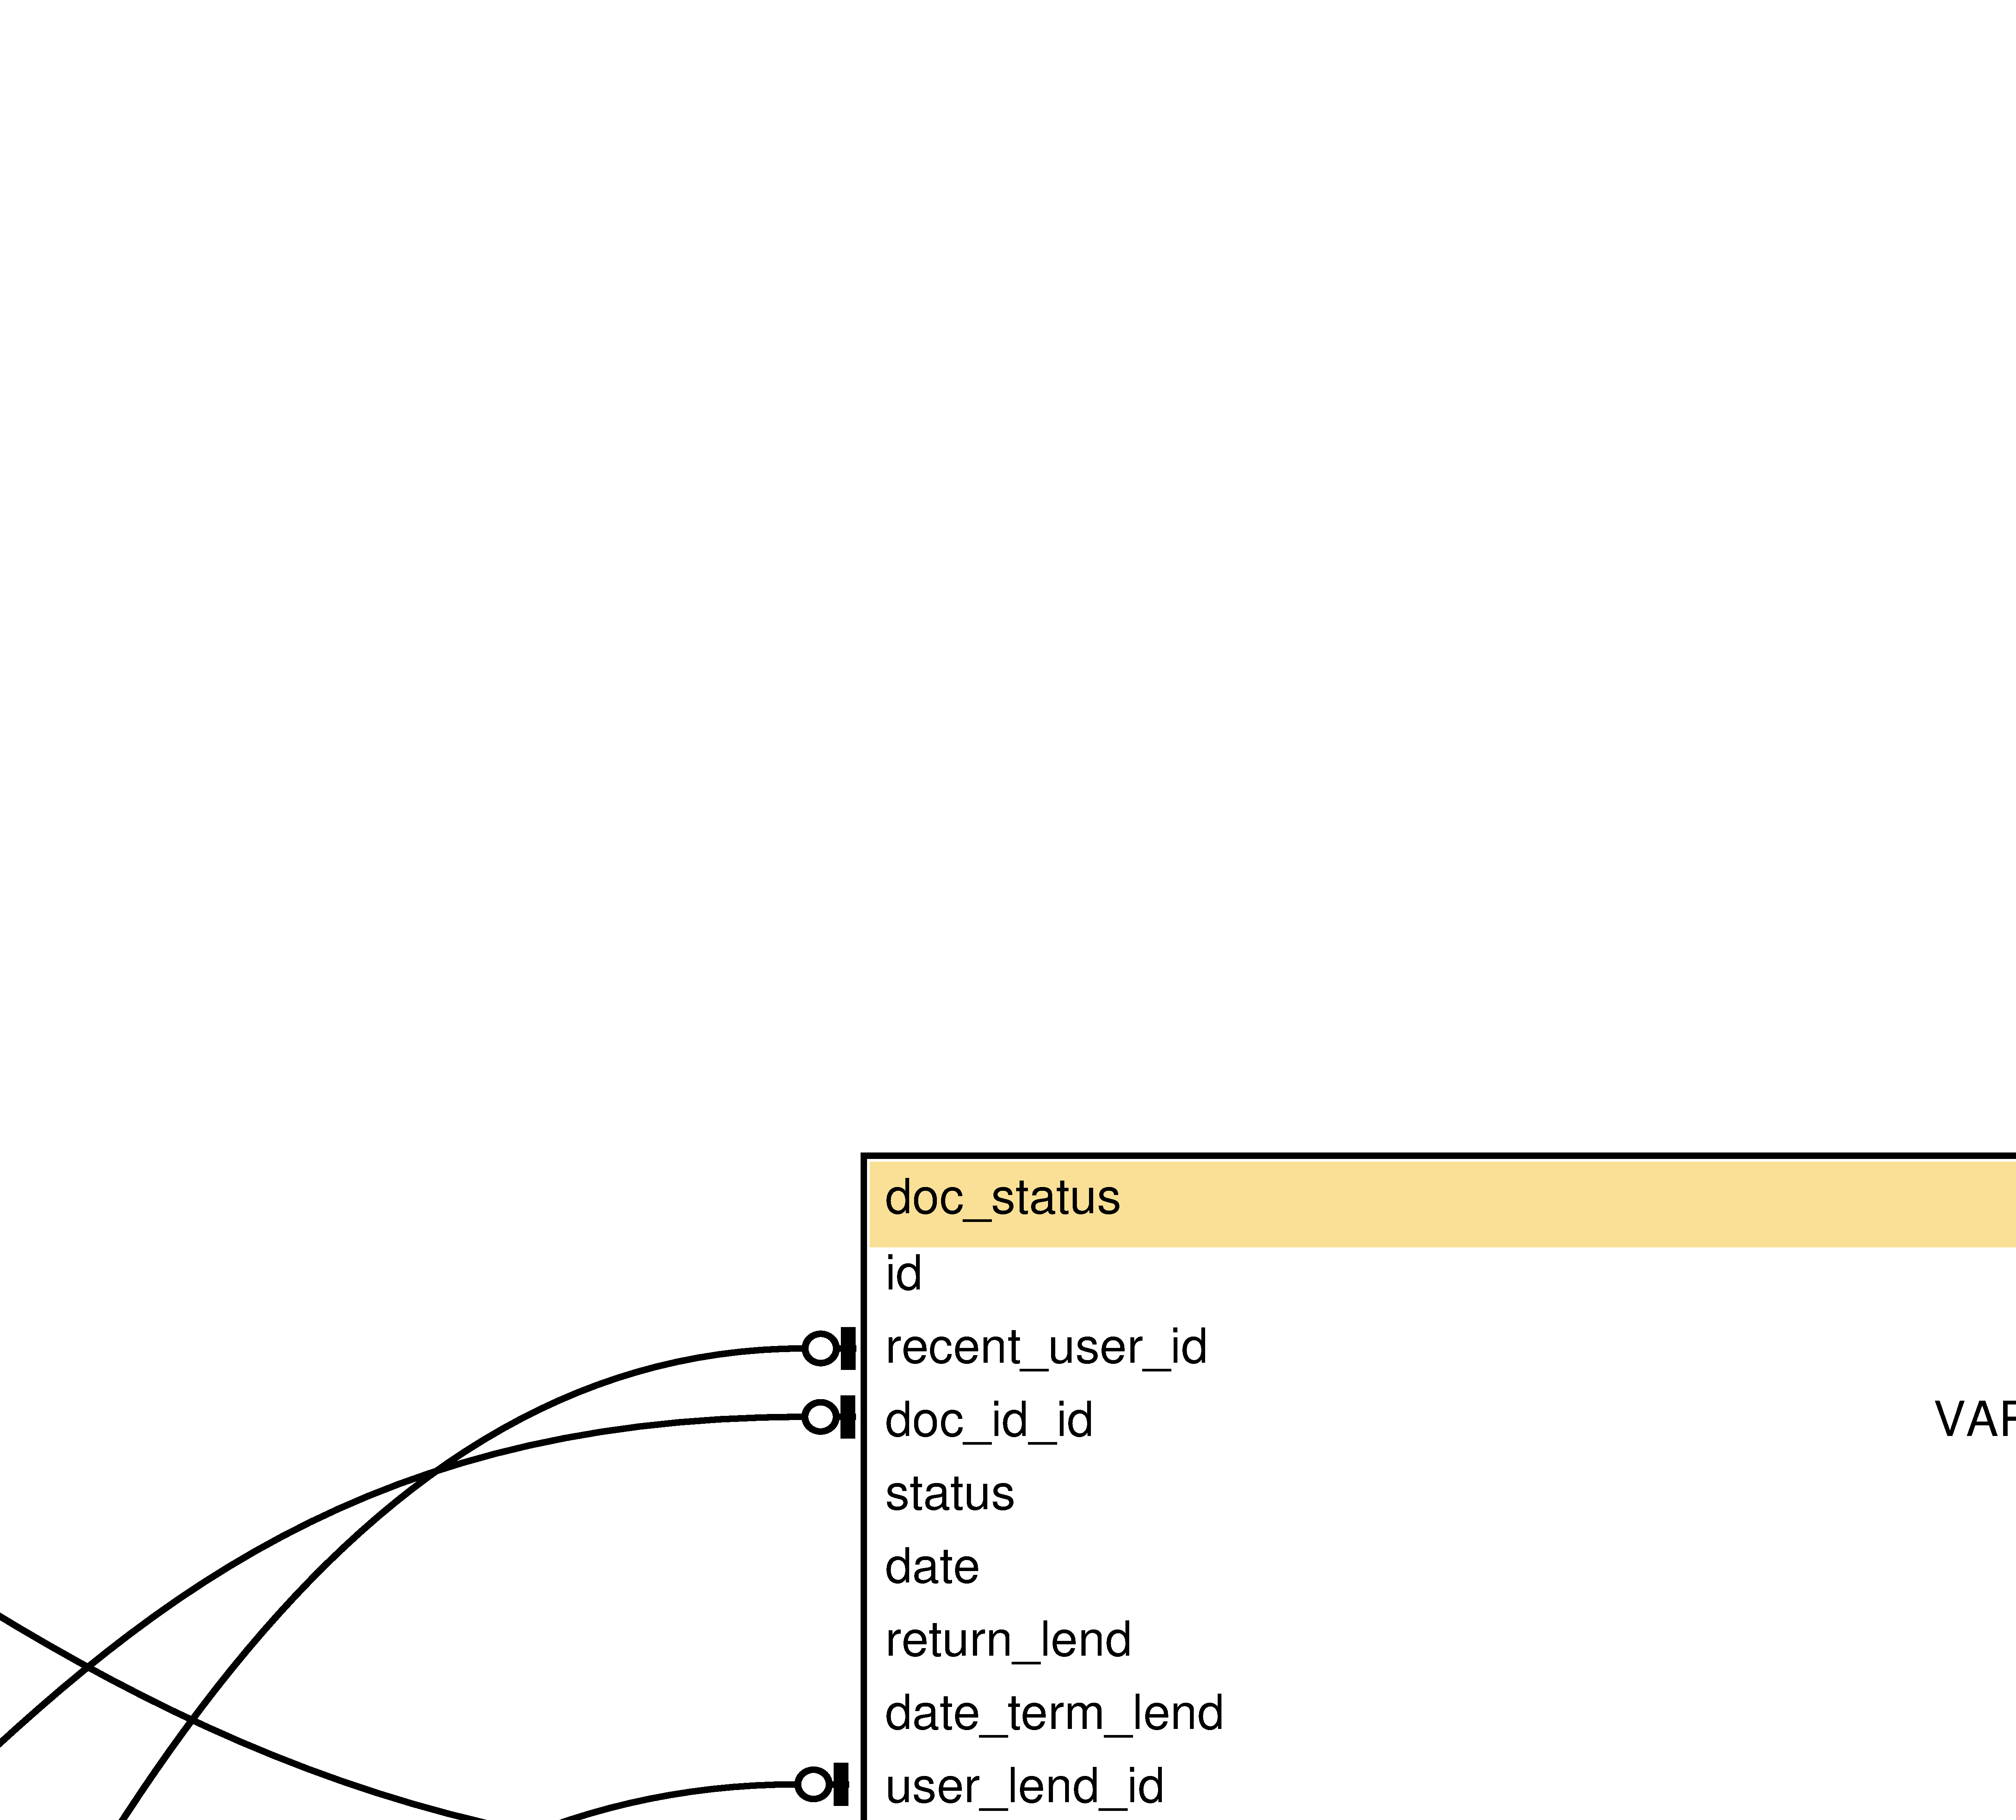
\includegraphics[width=0.8\linewidth]{bilder/database-wirelib.pdf}
\caption{Datenbankmodell}
\label{fig:DBDiagramm}
\end{figure}

Das Diagramm gibt eine grobe Übersicht über die Struktur der zugrundeliegenden
relationalen Datenbank. Im Folgenden werden die beiden wichtigsten
Teilstrukturen der Datenbank für bessere Übersicht dargestellt.


\begin{figure}[!htb]
\includegraphics[width=0.8\linewidth]{bilder/database-wirelib_cluster-doc.pdf}
\caption{Datenbankmodell: Bibliothek}
\label{fig:DB_docDiagramm}
\end{figure}

Dieses Diagramm gibt eine Übersicht über alle Tabellen der Datenbank, die im
Zusammenhang mit der Bibliothek stehen. Die wichtigste Tabelle ist document, in
der die vorhandenen Dokumente eingetragen werden. In der Tabelle doc\_status
werden alle Statusänderungen eines Dokumentes festgehalten, einschließlich der
Ausleihe eines Dokumentes. Die Tabelle doc\_extra speichert zusätzliche Inhalte
eines Dokumentes, die aufgrund seltenen Gebrauchs nicht lohnen, in document
direkt aufgenommen zu werden. In der Tabelle emails werden die E-Mail-Templates
gespeichert, die verschickt werden, wenn die Ausleihfrist eines Dokumentes
abläuft oder in ähnlichen Fällen. Die Tabellen auth\_user und non\_user sind
in der Teilstruktur Benutzer und hier nur als Referenz gedacht zur besseren
Übersicht. Die verbleibenden Tabellen speichern trivialerweise den
beschriebenen Inhalt.


\begin{figure}[!htb]

\includegraphics[width=0.8\linewidth]{bilder/database-wirelib_cluster-user.pdf}
\caption{Datenbankmodell: Benutzer}
\label{fig:DB_UserDiagramm}
\end{figure}

Dieses Diagramm gibt eine Übersicht über alle Tabellen der Datenbank, die im
Zusammenhang mit Benutzerverwaltung stehen. Alle Tabellen, die in diesem Modell
mit dem Präfix \emph{auth\_} beginnen, sind von Django generiert und werden für
eine erleichterte Handhabung von Benutzern und Rechtevergabe genutzt. Tabellen
mit dem Präfix \emph{django\_} werden ebenfalls von Django generiert und dienen
dem Admin-Interface von Django und dem Session-Managment von eingeloggten
Benutzern. Die Tabelle non\_user ist für Nutzer gedacht, die nicht am Institut
für Wissenschaftliches Rechnen arbeiten und trotzdem ein Dokument ausleihen
wollen. Sie haben so keine Möglichkeit, sich auf der Webseite einzuloggen,
können aber trotzdem Dokumente ausleihen. Die Tabellen tel\_user und
tel\_non\_user werden benötigt, um Telefonnumern zu Benutzern zu speichern.
user\_profile ist zur Erweiterung der Django-Tabelle auth\_user, um auch
Adressen speichern zu können.

% Eigenes Klassendiagramm einsetzen
\section{Erl\"auterung}

\begin{tabular}[ht]{|l||c|c|}
  \hline
  Entit\"at & \multicolumn{2}{c|}{Beziehungen} \\
  \hline\hline\hline
  
  author  & Name der Beziehung &  Kardinalit\"at\\
  \hline\hline
  document\_authors & hat geschrieben & 1,n \\
  \hline\hline\hline
  
  document\_authors & Name der Beziehung & Kardinalität\\
  \hline\hline
  author & wurde geschrieben von & 1\\
  \hline
  document & hat geschrieben & 1\\
  \hline\hline\hline
  
  document: & Name der Beziehung & Kardinalität\\
  \hline\hline
  document\_authors & wurde geschrieben von & 1,n\\
  \hline
  category & gehört zur Kategorie & 1\\
  \hline
  publisher & wurde veröffentlicht von & 1\\
  \hline
  keywords & besitzt die Schlüsselwörter & n\\  
  \hline
  doc\_extra & besitzt die Extrafelder & n\\
  \hline
  doc\_status & hat den Status/verliehen an & n\\
  \hline\hline\hline
  
  keywords:  & Name der Beziehung &  Kardinalit\"at\\
  \hline\hline
  document & gehört zum Dokument & 1 \\
  \hline\hline\hline
  
  publisher:  & Name der Beziehung &  Kardinalit\"at\\
  \hline\hline
  document & hat veröffentlicht & 1,n \\
  \hline\hline\hline
  
  category:  & Name der Beziehung &  Kardinalit\"at\\
  \hline\hline
  document & enthält & n \\
  \hline\hline\hline
  
  doc\_extra:  & Name der Beziehung &  Kardinalit\"at\\
  \hline\hline
  document & gehört zu & 1 \\
  \hline\hline\hline
  
  doc\_status: & Name der Beziehung & Kardinalität\\
  \hline\hline
  document & gehört zum Dokument & 1\\
  \hline
  auth\_user & wurde geändert von & 1\\
  \hline
  auth\_user & wurde ausgeliehen von & 0,1\\
  \hline
  non\_user & wurde weitergegeben an & 0,1\\
  \hline\hline\hline
  
  non\_user: & Name der Beziehung & Kardinalität\\
  \hline\hline
  doc\_status & entlieh & 1,n\\
  \hline
  tel\_non\_user & hat die Telefonnummern & 1,n\\
  \hline\hline\hline
  
  tel\_non\_user:  & Name der Beziehung &  Kardinalit\"at\\
  \hline\hline
  non\_user & gehört zu & 1 \\
  \hline
\end{tabular}

\begin{tabular}[ht]{|l||c|c|}
  \hline
  Entit\"at & \multicolumn{2}{c|}{Beziehungen} \\
  \hline\hline\hline
    
  auth\_user: & Name der Beziehung & Kardinalität\\
  \hline\hline
  user\_profile & wohnt & 1\\
  \hline
  tel\_user & hat die Telefonnumern & 1,n\\
  \hline
  auth\_user\_user\_permissions & hat die Rechte & n\\
  \hline
  doc\_status & änderte den Status & n\\  
  \hline
  doc\_status & leiht/bürgt gerade für & n\\
  \hline
  django\_admin\_log & aktualisiert & n\\
  \hline
  auth\_message & bekam & n\\
  \hline\hline\hline
  
  tel\_user:  & Name der Beziehung &  Kardinalit\"at\\
  \hline\hline
  auth\_user & gehört zu & 1 \\
  \hline\hline\hline 
  
  auth\_message: & Name der Beziehung &  Kardinalit\"at\\
  \hline\hline
  auth\_user & gesendet an & 1 \\
  \hline\hline\hline 
  
  user\_profile:  & Name der Beziehung &  Kardinalit\"at\\
  \hline\hline
  auth\_user & Anschrift von & 1 \\
  \hline\hline\hline
  
  auth\_user\_groups:  & Name der Beziehung &  Kardinalit\"at\\
  \hline\hline
  auth\_user & der User & 1 \\
  \hline
  auth\_group & gehört zur Gruppe & 1 \\
  \hline\hline\hline
  
  auth\_group: & Name der Beziehung &  Kardinalit\"at\\
  \hline\hline
  auth\_user\_groups & besitzt die Mitglieder & n \\
  \hline
  auth\_group\_permissions & hat die Rechte & n \\
  \hline\hline\hline 

  auth\_group\_permissions: & Name der Beziehung &  Kardinalit\"at\\
  \hline\hline
  auth\_group & die Gruppe & 1 \\
  \hline
  auth\_permission & hat das Recht & 1 \\
  \hline\hline\hline 
  
  auth\_user\_user\_permissions:  & Name der Beziehung &  Kardinalit\"at\\
  \hline\hline
  auth\_user & der User & 1 \\
  \hline
  auth\_permission & hat das Recht & 1 \\
  \hline\hline\hline 
  
  auth\_permission:  & Name der Beziehung &  Kardinalit\"at\\
  \hline\hline
  auth\_user\_user\_permissions & der User hat  & n \\
  \hline
  auth\_group\_permissions & die Gruppe hat & n \\
  \hline
  django\_content\_type & referenziert & 1 \\
  \hline
\end{tabular}

\begin{tabular}[ht]{|l||c|c|}
  \hline
  Entit\"at & \multicolumn{2}{c|}{Beziehungen} \\
  \hline\hline\hline
  
  django\_admin\_log:  & Name der Beziehung &  Kardinalit\"at\\
  \hline\hline
  auth\_user & getätigt von  & 1 \\
  \hline
  django\_content\_type & referenziert & 1 \\
  \hline\hline\hline
  
  django\_content\_type:  & Name der Beziehung &  Kardinalit\"at\\
  \hline\hline
  auth\_permission & stellt Referenz  & n \\
  \hline
  django\_admin\_log & ändert & n \\
  \hline\hline\hline
\end{tabular}
